\documentclass{llncs}
\usepackage{llncsdoc}
\usepackage{color,soul}
\usepackage{times}
\usepackage{epsfig}
\usepackage{graphicx}
\usepackage{amsmath}
\usepackage{amssymb}
\usepackage{textcomp}
\usepackage{graphicx}
\usepackage{pslatex}
\usepackage{subfigure}
\usepackage{amsmath}
\usepackage{amssymb}
\usepackage{tikz}
\usepackage{marvosym}
\usepackage{wasysym}
\usepackage{times}
\usepackage{epsfig}
\usepackage{tabularx}
\usepackage{enumitem}
\usepackage{sidecap}
\usepackage{verbatim}
\usepackage{makecell}
%\usepackage{titling}

%\setlength{\droptitle}{-11em}   % This is your set screw
% If you comment hyperref and then uncomment it, you should delete
% egpaper.aux before re-running latex.  (Or just hit 'q' on the first latex
% run, let it finish, and you should be clear).
\usepackage[pagebackref=true,breaklinks=true,letterpaper=true,colorlinks,bookmarks=false]{hyperref}

\def\httilde{\mbox{\tt\raisebox{-.5ex}{\symbol{126}}}}
% Pages are numbered in submission mode, and unnumbered in camera-ready
\usepackage[parfill]{parskip}
  \title{Vision-Based Classification of Developmental Disorders Using Eye-Movements  \vspace{-1em}}
    \author{
    	Guido Pusiol\inst{1} \and Andre Esteva\inst{2}
  	\and Scott Hall \inst{3}
	\and Michael Frank \inst{4},\\
	 Arnold Milstein\inst{5}
	\and Li Fei-Fei \inst{1}
	}
\index{Pusiol,Guido}
\index{Esteva,Andre}
\index{Hall,Scott}
\index{Milstein,Arnold}
\index{Li,Fei-Fei}
   \institute{Dept. of Computer Science, Stanford University, USA\\
  	\and
  	Dept. of Electrical Engineering, Stanford University, USA\\
  	\and
  	Dept. of Psychiatry, Stanford University, USA\\
	\and
  	Dept. of Psychology, Stanford University, USA \\
	\and
  	Dept. of Medicine, Stanford University, USA \\
  }
  \begin{document}

   \maketitle
  \begin{abstract}
   \vspace{-0.5em}
    This paper proposes a system for fine-grained classification of developmental disorders via measurements of individuals' eye-movements using multi-modal visual data. While the system is engineered to solve a psychiatric problem, we believe the underlying principles and general methodology will be of interest not only to psychiatrists but to researchers and engineers in medical machine vision. The idea is to build features from different visual sources that capture information not contained in either modality. Using an eye-tracker and a camera in a setup involving two individuals speaking, we build temporal attention features that describe the semantic location that one person is focused on relative to the other person's face. In our clinical context, these temporal attention features describe a patient's gaze on finely discretized regions of an interviewing clinician's face, and are used to classify their particular developmental disorder. 
  \end{abstract}
  
  %%%%%%%%% BODY TEXT
  \vspace{-2.5em}
  \section{Introduction}
  \vspace{-1em}
 Autism Spectrum Disorders (ASD) is an important developmental disorder with both increasing prevalence and substantial social impact. Significant effort is spent on early diagnosis, which is critical for proper treatment. In addition, ASD is also a highly heterogeneous disorder, making diagnosis especially problematic. Today, identification of ASD requires a set of cognitive tests and hours of clinical evaluations that involve extensively testing participants and observing their behavioral patterns (e.g. their social engagement with others). Computer-assisted technologies to identify ASD are thus an important goal, potentially decreasing diagnostic costs and increasing standardization.

  In this work, we focus on Fragile-X-Syndrome (FXS). FXS is the most common known genetic cause of autism \cite{Hagerman:2008wg}, affecting approximately 100,000 people in the United States. Individuals with FXS exhibit a set of developmental and cognitive deficits including impairments in executive functioning, visual memory and perception, social avoidance, communication impairments and repetitive behaviors \cite{Sullivan:2007gz}. In particular, as in ASD more generally, eye-gaze avoidance during social interactions with others is a salient behavioral feature of individuals with FXS. FXS is an important case study for ASD because it can be diagnosed easily as a single-gene mutation. For our purposes, the focus on FXS means that ground-truth diagnoses are available and heterogeneity of symptoms in the affected group is reduced.

  Maintaining appropriate social gaze is critical for language development, emotion recognition, social engagement, and general learning through shared attention \cite{Csibra:2006wf}. Previous studies \cite{klin2002,Golarai} suggest that gaze fluctuations play an important role in the characterization of individuals in the autism spectrum. In this work, we study the underlying patterns of visual fixations during dyadic interactions. In particular we use those patterns to characterize different developmental disorders.

  We address two problems. The first challenge is to build new features to characterize fine behaviors of participants with developmental disorders. We do this by exploiting computer vision and multi-modal data to capture detailed visual fixations during dyadic interactions. The second challenge is to use these features to build a system capable of discriminating between developmental disorders. The remainder of the paper is structured as follows: In section 2, we discuss prior work. In section 3, we describe the raw data: its collection and the sensors used. In section 4, we describe the built features and analyze them. In section 5, describe our classification techniques. In section 5, we describe the experiments and results. In section 6 we discuss the results.

  \begin{figure}
      \subfigure[]{
    \includegraphics[width=0.50\textwidth]{figures/pull.png}
    }
    \hfill
    \subfigure[]{
    \includegraphics[width=0.40\columnwidth]{figures/Real.png}
    }


    \label{fig:pull_figure}
    \caption{(a) We study social interactions between a participant with a mental impairment and an interviewer, using multi-modal data from a remote eye-tracker and camera. The goal of the system is to achieve fine-grained classification of developmental disorders using this data. (b) A frame from videos showing the participant's view (participant's head is visible in the bottom of the frame). Eye-movements were tracked with a remote eye-tracker and mapped into the coordinate space of this video.
    }
  \end{figure}
  \vspace{-3em}
  %%%%%%% PREVIOUS WORK %%%%%%%%
  \section {Previous Work}
  \vspace{-1em}

  Pioneering work by Rehg et al. \cite{RAG33} shows the potential of using coarse gaze information to measure relevant behavior in children with ASD.
  However, this work does not address the issue of fine-grained classification between ASD and other disorders in an automated way. Our work thus extends this work to develop a means for disorder classification via multi-modal data.
   In addition, some previous efforts in the classification of developmental disorders such as epilepsy and schizophrenia have relied on using electroencephalogram (EEG) recordings \cite{Kumar}. These methods are accurate, but they require long recording times; in addition, the use of EEG probes positioned over a participant's scalp and face can limit applicability to developmental populations. Meanwhile, eye-tracking has long been used to study autism \cite{Boraston,hashemi}, but we are not aware of an automated system for inter-disorder assessment using eye-tracking such as the one proposed here.

  \vspace{-1.5em}
  \section{Dataset}
  \vspace{-1.5em}
 Our dataset consists of 70 videos of an clinician interviewing a participant, overlaid with the participant's point of gaze (as measure by a remote eye-tracker), first reported in \cite{hall2015quantifying}.

 The participants were diagnosed with either an idiopathic developmental disorder (DD) or Fragile-X-Syndrome (FXS). DD
presents similar autistic symptoms to FXS, but does not have FXS or any other known genetic syndrome.There are known gender-related behavioral differences between FXS participants, so we further subdivided this group by gender into males (FXS-M) and females (FXS-F). There were no gender-related behavioral differences in the DD group, and genetic testing confirmed that DD participants did not have FXS.

  Participants were between 12 and 28 years old, with 51 FXS participants (32 male, 19 female) and 19 DD participants. The two groups were well-matched on chronological and developmental age, and had similar mean scores on the Vineland Adaptive Behavior Scales (VABS), a well-established measure of developmental functioning. The average score was 58.5 ($SD = 23.47$) for individuals with FXS and 57.7 ($SD= 16.78$) for controls, indicating that the level of cognitive functioning in both groups was 2 -- 3 SDs below the typical mean.
  
  Participants were each interviewed by a clinically-trained experimenter. In our setup the camera was placed behind the patient and facing the interviewer. Figure \ref{fig:pull_figure} depicts the configuration of the interview, and of the physical environment. Eye-movements were recorded using a Tobii X120 remote corneal reflection eye-tracker, with time-synchronized input from the scene camera. The eye-tracker was spatially calibrated to the remote camera via the patient looking at a known set of locations prior to the interview.

  \vspace{-2 em}
  \section{Visual Fixation Features}
  \vspace{-1 em}
  \label{sec:feature_extraction}
A goal of our work is to design features that simultaneously provide insight into these disorders and allow for accurate classification between them. These features are the building blocks of our system, and the key challenge is engineering them to properly distill the most meaningful parts out of the raw eye-tracker and video footage. We capture the participant's point of gaze and its distribution over the interviewer's face, 5 times per second during the whole interview. There are 6 relevant regions of interest: \textit{nose, left eye, right eye, mouth, jaw, outside face}. The precise detection of these fine-grained features enables us to study small changes in participants' fixations at scale.

For each video frame, we detected a set of 69 landmarks on the interviewer's face using a part-based model \cite{dpmface}. Figure \ref{fig:pull_figure} shows examples of landmark detections. In total, we processed 14,414,790 landmarks. 
We computed 59K, 56K and 156K frames for DD, FXS-Female, and FXS-Male groups respectively. We evaluated a sample of 1K randomly selected frames, out of which only a single frame was incorrectly annotated. We mapped the eye-tracking coordinates to the facial landmark coordinates with a linear transformation. Our features take the label of the cluster (e.g. jaw) holding the closest landmark to the participant point of gaze. We next present some descriptive analyses of these data.

\paragraph{Feature granularity.} We want to analyze the relevance of our fine grained attention features.
Participants---especially those with FXS---spent only a fraction of the time looking at the interviewer's face. Analyzing the time series data of when individuals are glancing at the face of their interviewer (see Figure \ref{fig:sticky}), we observe high inter-group participant's variance. For example, most of FXS-F individual sequences could be easily confused with the other groups.

 \begin{figure}[t]
    \subfigure[DD]{
    \includegraphics[width=1.4in,height= 1in]{figures/FXSF-face.png}
    }
     \hfill
     \subfigure[FXS-F]{
     \includegraphics[width=1.4in,height= 1in]{figures/DD-face.png}
    }
     \hfill
     \centering
    \subfigure[FXS-M]{
     \includegraphics[width=1.4in,height= 1in]{figures/FXSM-face.png}
     }
  \vspace{-1 em}
     \caption{Temporal analysis of attention to face. X axis represents time in frames (in increments of 0.2 seconds). Y axis represents each participant. Black dot represent time points when the participant was looking at the interviewer's face. White space signifies that they were not.}
    \label{fig:sticky}
    \vspace{-1 em}
   \end{figure}
   
Clinicians often express the opinion that the \emph{distribution} of fixations, not just the sheer lack of face fixations---seem related to the general autism phenotype \cite{klin2002,jones2013}. This opinion is supported by the distributions in Figure \ref{fig:histo}: DD and FXS-F are quite similar, whereas FXS-M is distinct. FXS-M focuses primarily on mouth (4) and nose (1) areas.
  
  \begin{figure}[h]
    \subfigure[DD]{
    \includegraphics[width=1.5in,height= 0.6in]{figures/semdd-face.png}
    }
    \hfill
    \subfigure[FXS-F]{
    \includegraphics[width=1.5in,height= 0.6in]{figures/semfemale-face.png}
    }
    \hfill
    \subfigure[FXS-M]{
    \includegraphics[width=1.5in,height= 0.6in]{figures/semmale-face.png}
    }
    \vspace{-1 em}
    \caption{Histograms of visual fixation for the various disorders. X-axis represents fixations, from left to right: nose (1), eye-left (2), eye-right (3), mouth (4), and jaw (5). The histograms are computed with the data of all participants. The non-face fixation is removed for visualization convenience. }
    \label{fig:histo}
   \vspace*{-\baselineskip}
  \end{figure}

  \paragraph{Attentional transitions.} In addition to the distribution of fixations, clinicians also believe that the \emph{sequence} of fixations describe underlying behavior. In particular, FXS participants often glance to the face quickly and then look away, or scan between non-eye regions. Figure \ref{fig:transitions} shows region-to-region transitions in a heatmap. There is a marked difference between the different disorders: Individuals with DD make more transitions, while those with FXS exhibit significantly less---congruent with the clinical intuition. The transitions between facial regions better identify the three groups than the transitions from non-face to face regions. FXS-M participants tend to swap their gaze quite frequently between mouth and nose, while the other two do not. DD participants exhibit much more movement between facial regions, without any clear preference. FXS-F patterns resemble DD, though the pattern is less pronounced.
  
  \begin{figure}[t]
    \subfigure[DD]{
    \includegraphics[width=1.5in,height= 0.7in]{figures/transdd.png}
    }
    \hfill
    \subfigure[FXS-F]{
    \includegraphics[width=1.5in,height= 0.7in]{figures/transfemale.png}
    }
    \hfill
    \subfigure[FXS-M]{
    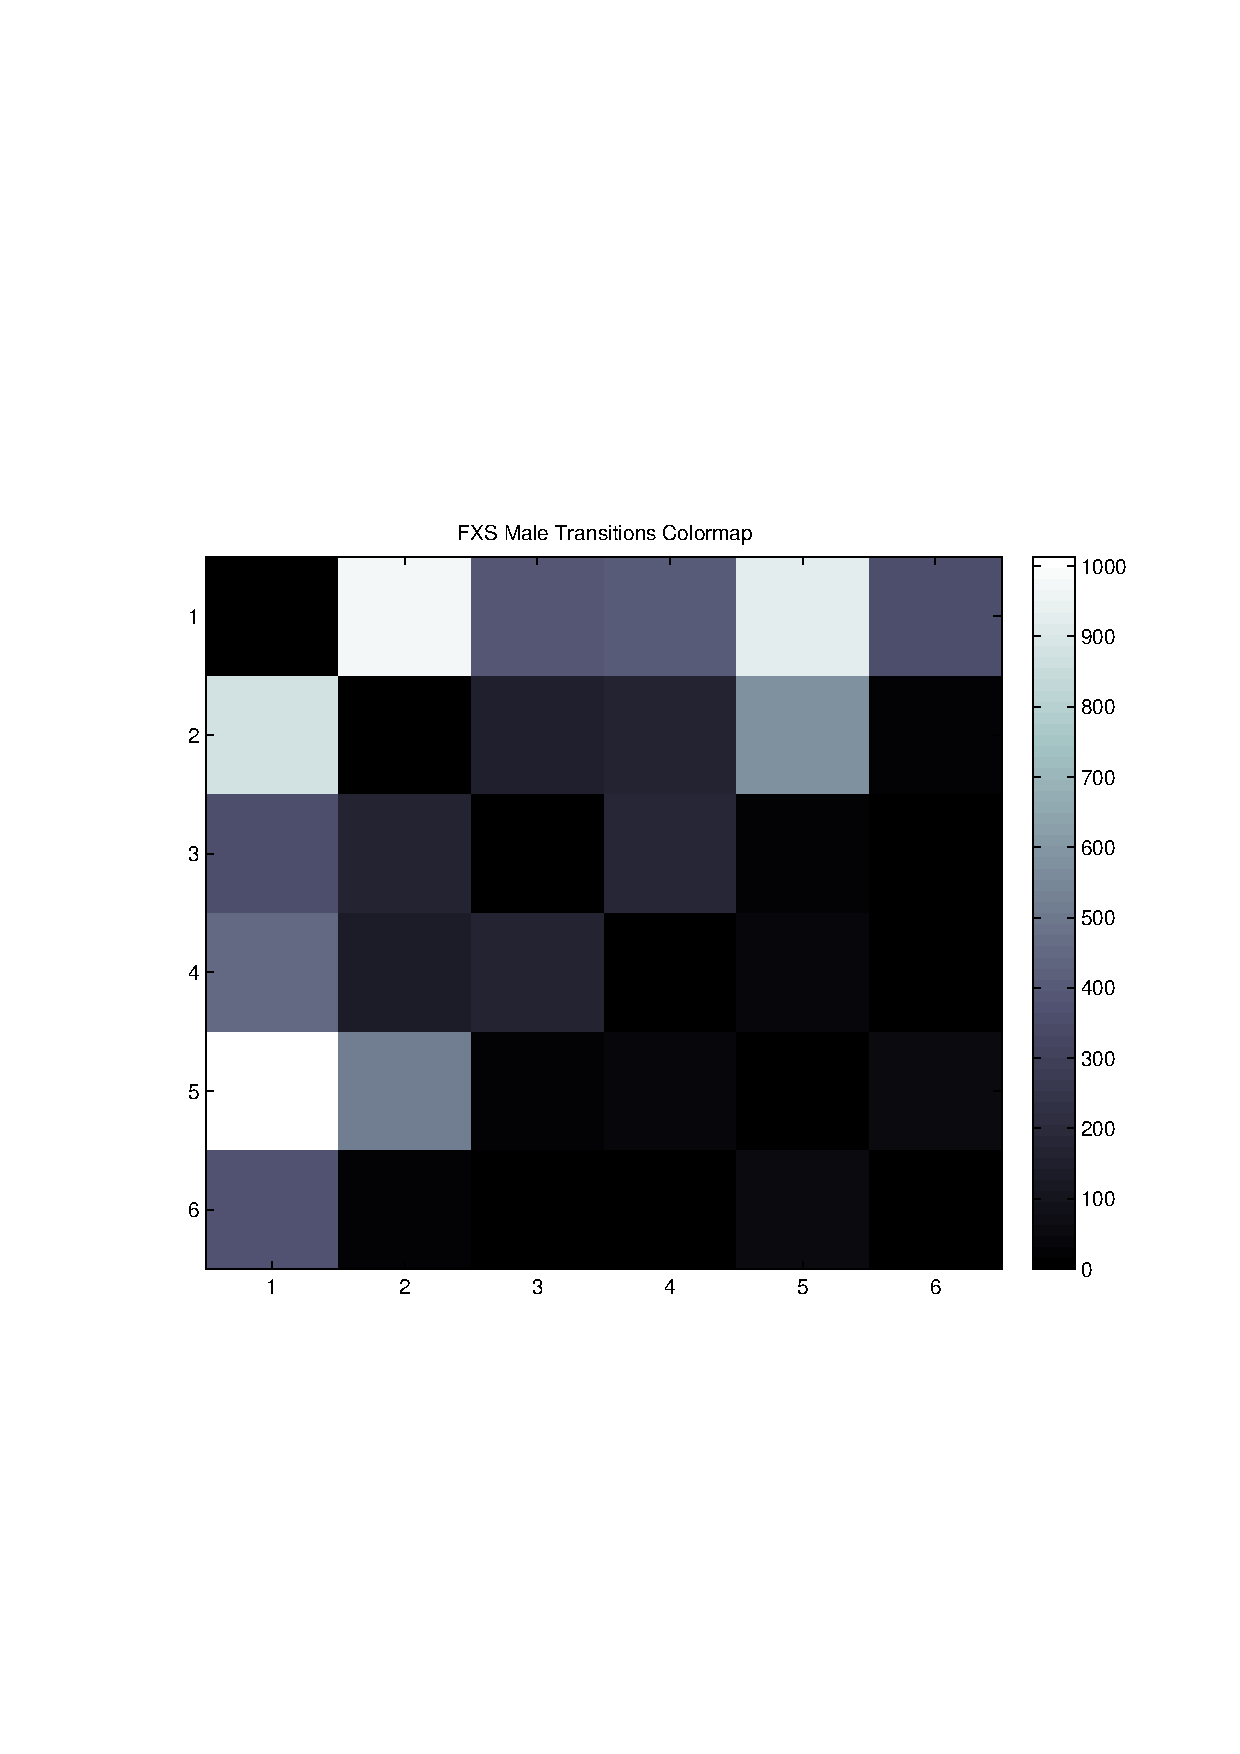
\includegraphics[width=1.5in,height= 0.7in]{figures/transmale.png}
    }
    \caption{Matrix of attentional transitions for each disorder. Each square $[ij]$ represents the aggregated number of times participants of each group transitioned attention from state $i$ to state $j$.  The axes represent the different states: non-face (0), nose (1), eye-left (2), eye-right (3), mouth (4), and jaw (5).}
    \label{fig:transitions}
    \vspace*{-\baselineskip}
  \end{figure}

  \paragraph{Approximate Entropy.} We next estimate Approximate Entropy ($ApEn$) analysis to provide a measure of how predictable a sequence is \cite{Restrepo:2014gs} . A lower entropy value indicates a higher degree of regularity in the signal. For each group (DD, FXS-Female, FXS-Male), we selected 15 random participants sequences. We compute $ApEn$ by varying $w$ (sliding window length). Figure \ref{fig:individual_entropy} depicts this analysis. We can see that there is great variance amongst individuals of each population, many sharing similar entropy with participants of other groups. The high variability of the data sequences makes them harder to classify.    
  \begin{figure}[h]
    \centering
    \subfigure[DD]{
    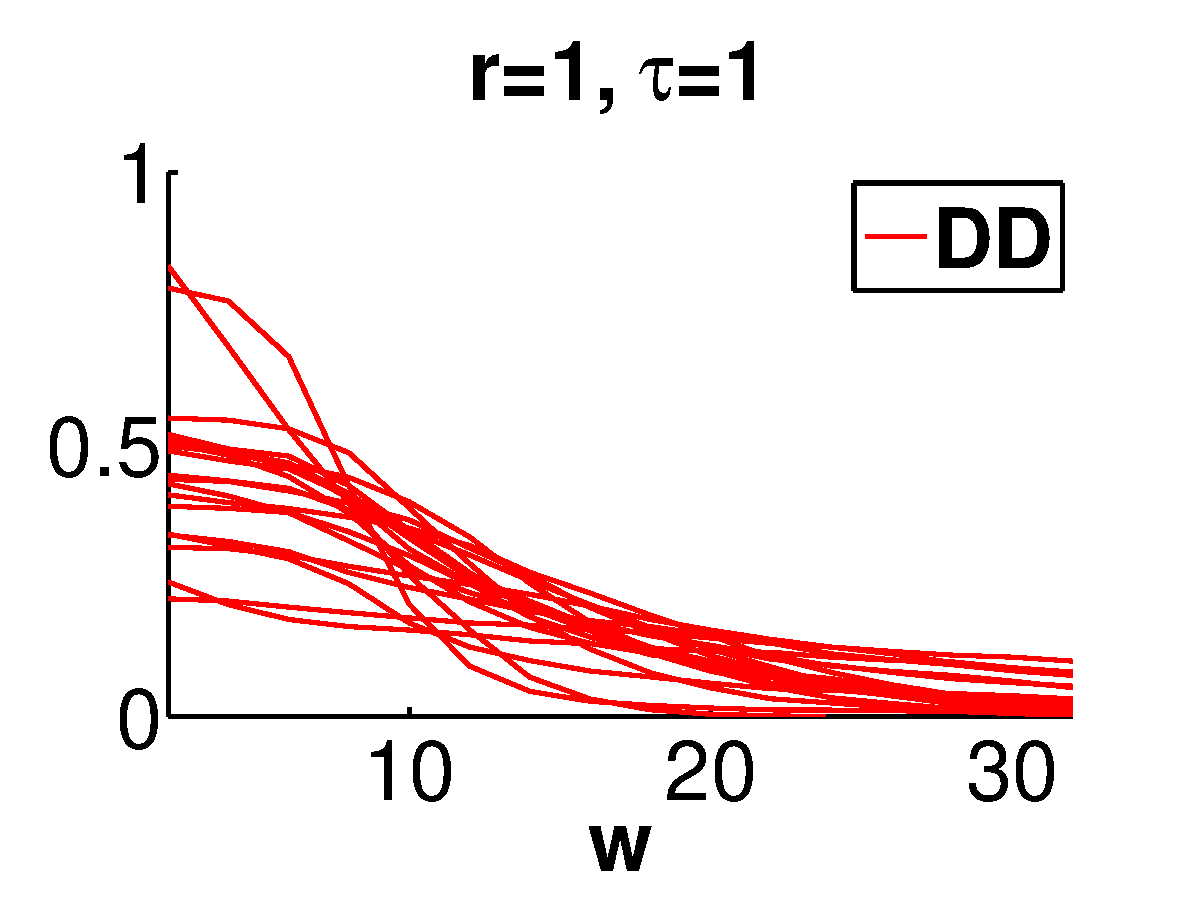
\includegraphics[width=1.5in,height= 1in]{figures/DDen}
    }
    \hfill
    \subfigure[FXS-F]{
    \includegraphics[width=1.5in,height= 1in]{figures/FXFen}
    }
    \hfill
    \subfigure[FXS-M]{
    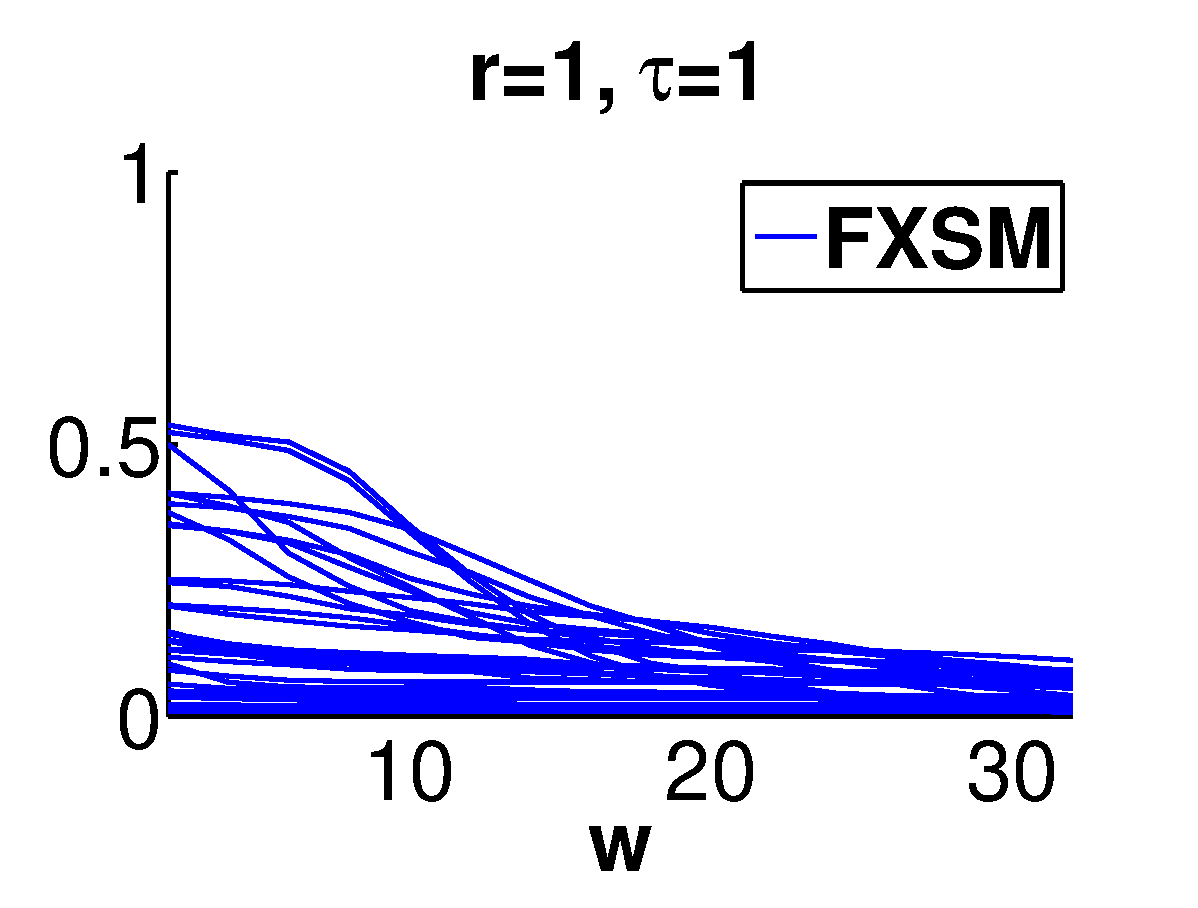
\includegraphics[width=1.5in,height= 1in]{figures/FXMen}
    }
    \caption{(a) - (c) Analysis of the $ApEn$ of the data per individual varying the window length parameter $w$. Y-axis is $ApEn$ and X-axis varies $w$. Each line represents one participant's data. We observe great variance among individuals.}
    \label{fig:individual_entropy}
    \vspace*{-\baselineskip}
\end{figure}

  \vspace*{-\baselineskip}
  \section{Classifiers}
  \vspace*{-\baselineskip}
  \label{sec:classification}
  The goal of this work is to create an end-to-end system for classification of developmental disorders from raw visual information. So far we have introduced features that capture social attentional information and analyzed their temporal structure. We next need to construct methods capable of utilizing these features to predict the specific disorder of the patient.
  \vspace*{-\baselineskip}
  \paragraph{Model (RNN).} The Recurrent Neural Network (RNN) is a generalization of feedforward neural networks to sequences. Our deep learning model is an adaptation of the attention-enhanced RNN architecture proposed by Hinton et al. \cite{NIPS2015_5635} (LSTM+A). The model has produced impressive results in other domains such as language modeling and speech processing. Our feature sequences fit this data profile. In addition, an encoder-decoder RNN architecture allows us to experiment with sequences of varying lengths in a cost-effective manner. Our actual models differ from LSTM+A in two ways. First, we have replaced the LSTM cells with GRU cells \cite{Cho}, which are are memory-efficient and could provide a better fit to our data \cite{JozefowiczZS15}. Second, our decoder produces a single output value (i.e. class). The decoder is a single-unit multi-layered RNN (without unfolding) and with a soft-max output layer. Conceptually it could be seen as a many-to-one RNN, but we present it as a configuration of \cite{NIPS2015_5635} given its proximity and our adoption of the attention mechanism.

For our experiments, we used 3 RNN configurations: RNN\_128: 3 layers of 128 units;  RNN\_256: 3 layers of 256 units; RNN\_512: 2 layers of 512  units. These parameters were selected considering our GPU memory allocation limitation.\\
We trained our models for a total of 1000 epochs. We used batches of sequences, SGD with momentum and max gradient normalization (0.5). 
\vspace*{-\baselineskip}
\paragraph{Other Classifiers.} We also trained shallow baseline classifiers. We engineer a convolutional neural network approach (CNN) that can exploit the local-temporal relationship of our data.  It is composed of one hidden layer of 6 convolutional units followed by point-wise sigmoidal nonlinearities. The feature vectors computed across the units are concatenated and fed to an output layer composed of an affinity transformation followed by another sigmoid function. We also trained support vector machines ({SVMs}), Naive Bayes ({NB}) classifiers, and Hidden Markov Models ({HMMs}). 
\vspace*{-\baselineskip}
\section{Experiments and Results}
\vspace*{-\baselineskip}
By varying the classification methods described in Section \ref{sec:classification} we perform a quantitative evaluation of the overall system.
We assume the gender of the patient is known, and select the clinically-relevant pair-wise classification experiments DD vs FXS-F and DD vs FXS-M. For the experiments we use 32 FXS-male, 19 FXS-female and 19 DD participants. To maintain equal data distribution in training and testing we build $S_{train}$ and and $S_{test}$ randomly shuffling participants of each class ensuring a 50\%/50\% distribution of the two participant classes over the sets. At each new training/testing fold the process is repeated so that the average classification results will represent the entire set of participants. We classify the developmental disorder of the participants, given their individual time-series feature data $p$, to evaluate the precision of our system. For N total participants, we create an 80\%/20\% training/testing dataset such that no participant's data is shared between the two datasets. For each experiment, we performed 10-fold cross validation where each fold was defined by a new random 80/20 split of the participants --about 80 participant's were tested per experiment.   
\vspace*{-\baselineskip}

\paragraph{Metric.}
We consider the binary classification of an unknown participant as having DD or FXS. We adopt a voting strategy where, given a patient's data $p=[f_1, f_2,....f_{T}]$, we classify all sub-sequences $s$ of $p$ of fixed length $w$ using a sliding-window approach. In our experiments, $w$ correspond to 3, 10, and 50 seconds of video footage. To predict the participant's disorder, we employ a max-voting scheme over each class. The predicted class $C$ of the participant is given by:
  \begin{equation}
    C = \underset{c \in \{C_1, C_2\}} {\operatorname{argmax}} \sum_{\text{sub-seq. } s}^{} \bold{1}(\text{Class}(s) = c)
  \end{equation}
  Where $C_1, C_2 \in \{\text{DD}, \text{FXS-F}, \text{FXS-M}\}$, $\text{Class}(s)$ is the output of a classifier given input $s$. We use 10 cross validation folds to compute the average classification precision.
\vspace*{-2em}
\paragraph{Results.} The results are reported in Table  \ref{table:profiler}. We find that the highest average precision is attained using the RNN.512 model with a 50 second time window. It classifies DD versus FXS-F with 0.86 precision and DD versus FXS-M with 0.91 precision. We suspect that the salient results produced by the RNN\_512 are related to its high capacity and its capability of representing complex temporal structures.

\begin{table}[t]
    \centering
    \resizebox{0.9\columnwidth}{!}{%
    %\resizebox*{!}{\dimexpr\textheight-2\baselineskip\relax}{%
     \begin{tabular}{c|c|c|c}
      & window length & DD vs FXS-female (precision) & DD vs FXS-male (precision)\\
      \hline
      SVM  & 3   & 0.65 & 0.83\\
      & 10 & 0.65 & 0.80 \\
      & 50 & 0.55 & 0.85 \\
      
      \hline
      N.B   & 3  & 0.60 & 0.85\\
      & 10 & 0.60 & 0.87\\
      & 50 & 0.60 & 0.75\\

      \hline
      HMM & 3  & 0.67 & 0.81\\
      & 10 & 0.66 & 0.82\\
      & 50 & 0.68 & 0.74\\

      \hline
      CNN & 3 & 0.68 & 0.82 \\
      & 10 & 0.68 & 0.90\\
      & 50 & 0.55 & 0.77\\

      \hline
      RNN\_128  & 3 &  0.69 & 0.79 \\
      RNN\_250 & 10 &   0.79 &  0.81\\
      RNN\_512 &  50 & {\bf 0.86} & {\bf 0.91}
      \\
    \end{tabular}
    }
    \caption{Comparison of precision of our system against other classifiers. Columns denote pairwise classification precision of participants for DD vs FXS-female and DD vs FXS-male binary classification. Classifiers are run on 3,10, and 50 seconds time windows. We compare the system classifier, RNN to CNN, SVM, NB, and HMM algorithms.}
    \label{table:profiler}
    \vspace*{-2.5em}
  \end{table}
  
\vspace*{-\baselineskip}
\section{Conclusion}
\vspace*{-\baselineskip}
We hereby demonstrate the use of computer vision and machine learning techniques in a cost-effective system for assistive diagnosis of developmental disorders that exhibit visual phenotypic expression in social interactions. Data of experimenters interviewing participants with developmental disorders was collected using video and a remote eye-tracker. We built visual features corresponding to fine grained attentional fixations, and developed classification models using these features to discern between FXS and idiopathic developmental disorder. Despite finding a high degree of variance and noise in the signals used, our high accuracies imply the existence of temporal structures in the data.

This work serves as a proof of concept of the power of modern computer vision systems in assistive development disorder diagnosis. We are able to provide a high-probability prediction about specific developmental diagnoses based on a short eye-movement recording. This system, along with similar ones, could be leveraged for remarkably faster screening of individuals. Future work will consider extending this capability to a greater range of disorders and improving the classification accuracy.
  \vspace*{-\baselineskip}
  % {\footnotesize
  \bibliographystyle{splncs03}
  \bibliography{fxs-miccai}
  % }
\end{document}
